% ============================================================
% PromptForge -- Presentation Slides
% LaTeX Beamer -- Academic/Professional Style
%
% Compile with:
%   pdflatex slides.tex
%   pdflatex slides.tex   (run twice for TOC/refs)
%
% Required packages (all in standard TeX Live / MiKTeX / Overleaf):
%   beamer, xcolor, listings, booktabs, tikz, fontenc, inputenc
% ============================================================

\documentclass[aspectratio=169, 12pt]{beamer}

% -- Theme -------------------------------------------------------------------
\usetheme{Madrid}
\usecolortheme{whale}

% -- Custom colour palette (navy + blue -- matches the dashboard) ------------
\definecolor{pfnavy}{RGB}{30, 58, 95}
\definecolor{pfblue}{RGB}{37, 99, 235}
\definecolor{pflight}{RGB}{239, 246, 255}
\definecolor{pfgray}{RGB}{100, 116, 139}
\definecolor{pfgreen}{RGB}{5, 150, 105}
\definecolor{pfred}{RGB}{220, 38, 38}

\setbeamercolor{palette primary}{bg=pfnavy, fg=white}
\setbeamercolor{palette secondary}{bg=pfblue, fg=white}
\setbeamercolor{palette tertiary}{bg=pfnavy, fg=white}
\setbeamercolor{palette quaternary}{bg=pfnavy, fg=white}
\setbeamercolor{structure}{fg=pfblue}
\setbeamercolor{section in toc}{fg=pfnavy}
\setbeamercolor{frametitle}{bg=pfnavy, fg=white}
\setbeamercolor{title}{fg=white}
\setbeamercolor{block title}{bg=pfblue, fg=white}
\setbeamercolor{block body}{bg=pflight, fg=pfnavy}
\setbeamercolor{alerted text}{fg=pfred}
\setbeamercolor{example text}{fg=pfgreen}

% -- Typography --------------------------------------------------------------
\usepackage[T1]{fontenc}
\usepackage[utf8]{inputenc}
\usepackage{helvet}
\renewcommand{\familydefault}{\sfdefault}
\setbeamerfont{title}{size=\LARGE, series=\bfseries}
\setbeamerfont{frametitle}{size=\large, series=\bfseries}
\setbeamerfont{block title}{size=\normalsize, series=\bfseries}

% -- Packages ----------------------------------------------------------------
\usepackage{booktabs}
\usepackage{listings}
\usepackage{tikz}
\usepackage{graphicx}
\usepackage{array}
\usepackage{multirow}
\usepackage{xcolor}
\usepackage{textcomp}   % for \textrightarrow

% -- Code listing style ------------------------------------------------------
\lstset{
    basicstyle=\ttfamily\footnotesize,
    keywordstyle=\color{pfblue}\bfseries,
    commentstyle=\color{pfgray},
    stringstyle=\color{pfgreen},
    backgroundcolor=\color{pflight},
    frame=single,
    rulecolor=\color{pfblue},
    breaklines=true,
    showstringspaces=false,
    numbers=none,
    % Disable special character handling to avoid UTF-8 issues inside listings
    extendedchars=false,
    literate={->}{$\rightarrow$}{2}
             {=>}{$\Rightarrow$}{2},
}

% -- Beamer settings ---------------------------------------------------------
\setbeamertemplate{navigation symbols}{}
\setbeamertemplate{footline}{
  \leavevmode
  \hbox{
    \begin{beamercolorbox}[wd=.4\paperwidth,ht=2.5ex,dp=1ex,center]{palette primary}
      \usebeamerfont{author in head/foot}\insertshortauthor
    \end{beamercolorbox}
    \begin{beamercolorbox}[wd=.4\paperwidth,ht=2.5ex,dp=1ex,center]{palette secondary}
      \usebeamerfont{title in head/foot}\insertshorttitle
    \end{beamercolorbox}
    \begin{beamercolorbox}[wd=.2\paperwidth,ht=2.5ex,dp=1ex,center]{palette primary}
      \insertframenumber{} / \inserttotalframenumber
    \end{beamercolorbox}
  }
  \vskip0pt
}

% -- Metadata ----------------------------------------------------------------
\title[PromptForge]{PromptForge: An Interactive Prompt Engineering Evaluation Laboratory}
\subtitle{Demonstrating Measurable Impact of Prompt Design on LLM Output Quality}
\author[Your Name]{Your Name \\ \texttt{your.email@institution.edu}}
\institute{Department of Computer Science \\ Your Institution}
\date{\today}

% ============================================================
\begin{document}
% ============================================================

% -- Slide 1: Title ----------------------------------------------------------
\begin{frame}
  \titlepage
\end{frame}

% -- Slide 2: Outline --------------------------------------------------------
\begin{frame}{Outline}
  \tableofcontents
\end{frame}

% ============================================================
\section{Problem Statement}
% ============================================================

% -- Slide 3: The Problem ----------------------------------------------------
\begin{frame}{The Problem: Same Model, Wildly Different Results}
  \begin{columns}[T]
    \begin{column}{0.55\textwidth}
      \begin{itemize}
        \setlength\itemsep{0.6em}
        \item Large Language Models are powerful -- but output quality varies enormously
        \item Most users treat LLMs as black boxes and write poor prompts
        \item A bad prompt vs.\ a good prompt on the \textbf{same model} can differ
              by \textcolor{pfblue}{\textbf{60--70\%}} in quality
        \item No standard way to \textbf{compare}, \textbf{measure},
              or \textbf{teach} prompt engineering
      \end{itemize}
    \end{column}
    \begin{column}{0.42\textwidth}
      \begin{block}{Core Insight}
        The model hasn't changed.\\
        The training hasn't changed.\\
        The input is identical.\\[0.5em]
        \textbf{The prompt is the only variable.}
      \end{block}
    \end{column}
  \end{columns}
\end{frame}

% ============================================================
\section{Background: Prompt Engineering}
% ============================================================

% -- Slide 4: What is Prompt Engineering ------------------------------------
\begin{frame}{Prompt Engineering: The New Programming}
  \begin{columns}[T]
    \begin{column}{0.48\textwidth}
      \textbf{Traditional Programming}
      \begin{itemize}
        \item Write code to solve problems
        \item Compiled, deterministic
        \item Syntax errors caught at compile time
        \item Debugged with stack traces
      \end{itemize}
    \end{column}
    \begin{column}{0.48\textwidth}
      \textbf{Prompt Engineering}
      \begin{itemize}
        \item Write prompts to instruct AI
        \item Probabilistic, context-sensitive
        \item Logic errors visible only at runtime
        \item Debugged with prompt iteration
      \end{itemize}
    \end{column}
  \end{columns}
  \vspace{1em}
  \begin{alertblock}{Key Insight}
    Prompt engineering requires understanding model behaviour, designing evaluation
    metrics, and iterating systematically -- exactly like software engineering.
  \end{alertblock}
\end{frame}

% -- Slide 5: The 7 Strategies -----------------------------------------------
\begin{frame}{Seven Prompting Strategies}
  \small
  \begin{tabular}{@{}lll@{}}
    \toprule
    \textbf{Strategy} & \textbf{Core Idea} & \textbf{Best For} \\
    \midrule
    Zero-Shot         & Direct instruction, no examples            & Baseline measurement \\
    Few-Shot          & 2--3 labelled examples before the task     & Format-sensitive tasks \\
    Chain-of-Thought  & ``Think step-by-step''                     & Reasoning, analysis \\
    Role Prompting    & Assign expert persona                      & Domain expertise \\
    Structured Output & Enforce JSON schema                        & Downstream processing \\
    Self-Reflection   & Generate $\rightarrow$ critique $\rightarrow$ revise  & High-stakes accuracy \\
    Meta-Prompting    & Model designs its own prompt               & Novel/ambiguous tasks \\
    \bottomrule
  \end{tabular}
  \vspace{0.8em}
  \begin{exampleblock}{}
    Each strategy costs \textbf{nothing extra} -- they are just words.
    Their impact on output quality is measurable and dramatic.
  \end{exampleblock}
\end{frame}

% ============================================================
\section{System Architecture}
% ============================================================

% -- Slide 6: Architecture ---------------------------------------------------
\begin{frame}{PromptForge -- System Architecture}
  \begin{center}
  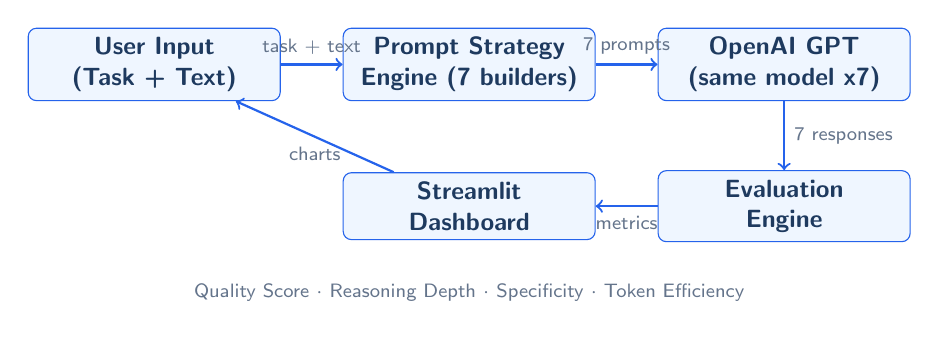
\begin{tikzpicture}[
    box/.style={rectangle, draw=pfblue, fill=pflight, rounded corners=3pt,
                minimum width=3.2cm, minimum height=0.85cm,
                font=\small\bfseries, align=center, text=pfnavy},
    arrow/.style={->, thick, color=pfblue},
    lbl/.style={font=\scriptsize, color=pfgray}
  ]
    \node[box] (input)  at (0,    0)   {User Input\\(Task + Text)};
    \node[box] (engine) at (4,    0)   {Prompt Strategy\\Engine (7 builders)};
    \node[box] (api)    at (8,    0)   {OpenAI GPT\\(same model x7)};
    \node[box] (eval)   at (8,  -1.8) {Evaluation\\Engine};
    \node[box] (dash)   at (4,  -1.8) {Streamlit\\Dashboard};

    \draw[arrow] (input)  -- node[lbl, above]{task + text} (engine);
    \draw[arrow] (engine) -- node[lbl, above]{7 prompts}   (api);
    \draw[arrow] (api)    -- node[lbl, right]{7 responses} (eval);
    \draw[arrow] (eval)   -- node[lbl, below]{metrics}     (dash);
    \draw[arrow] (dash)   -- node[lbl, below]{charts}      (input);

    \node[lbl, align=center] at (4, -2.9)
      {Quality Score $\cdot$ Reasoning Depth $\cdot$ Specificity $\cdot$ Token Efficiency};
  \end{tikzpicture}
  \end{center}
\end{frame}

% -- Slide 7: Tech Stack  [fragile] required for lstlisting ------------------
\begin{frame}[fragile]{Technical Stack}
  \begin{columns}[T]
    \begin{column}{0.48\textwidth}
      \textbf{Backend}
      \begin{itemize}
        \item Python 3.11+
        \item OpenAI SDK (\texttt{gpt-4o-mini})
        \item Custom NLP evaluation engine
        \item \texttt{python-dotenv} for secrets
      \end{itemize}
      \vspace{0.8em}
      \textbf{Frontend}
      \begin{itemize}
        \item Streamlit (interactive web UI)
        \item Plotly (bar, radar, scatter charts)
        \item Custom CSS (light professional theme)
      \end{itemize}
    \end{column}
    \begin{column}{0.48\textwidth}
      \textbf{Project Structure}
\begin{lstlisting}
promptforge/
  app.py
  prompts/
    strategies.py
    templates.py
  engine/
    llm_client.py
    evaluator.py
  data/
    examples.py
  .streamlit/
    config.toml
\end{lstlisting}
    \end{column}
  \end{columns}
\end{frame}

% ============================================================
\section{Evaluation Methodology}
% ============================================================

% -- Slide 8: Evaluation Metrics ---------------------------------------------
\begin{frame}{Evaluation Methodology -- Without Using Another LLM}
  \begin{block}{Design Goal}
    Quantify LLM output quality using \textbf{deterministic, fast, explainable} heuristics.
    Avoids circular evaluation (LLM judging LLM).
  \end{block}
  \vspace{0.4em}
  \small
  \begin{tabular}{@{}llrl@{}}
    \toprule
    \textbf{Metric}        & \textbf{Method}                          & \textbf{Max} & \textbf{Captures} \\
    \midrule
    Content Richness       & word\_count / 5, capped                  & 30 pts & Completeness \\
    Readability            & Flesch--Kincaid formula                  & 20 pts & Clarity \\
    Specificity            & Numbers + quotes + vocab diversity       & 20 pts & Concreteness \\
    Reasoning Depth        & Causal connectors (because, thus\ldots)  & 20 pts & Logical structure \\
    Structure Bonus        & Lists / headers / JSON keys present      &  5 pts & Organisation \\
    JSON Validity          & Parseable \{\} block in response         &  5 pts & Machine readability \\
    \midrule
    \textbf{Quality Score} & \textbf{Sum}                             & \textbf{100} & \\
    \bottomrule
  \end{tabular}
  \vspace{0.4em}
  \begin{alertblock}{Limitation (acknowledged)}
    Semantic correctness is \emph{not} verified -- only structural quality.
    High-quality structure does not guarantee factual accuracy.
  \end{alertblock}
\end{frame}

% ============================================================
\section{Live Demonstration}
% ============================================================

% -- Slide 9: Live Demo -------------------------------------------------------
\begin{frame}{Live Demonstration}
  \begin{center}
    \large\textbf{Launching PromptForge}
  \end{center}
  \vspace{0.5em}
  \begin{block}{Demo Setup}
    \begin{itemize}
      \item Task: \textbf{Code Review}
      \item Input: Python \texttt{login()} function with SQL Injection vulnerability
      \item Strategies: Zero-Shot, Chain-of-Thought, Role Prompting, Structured Output
    \end{itemize}
  \end{block}
  \vspace{0.5em}
  \textbf{Watch for:}
  \begin{itemize}
    \item Zero-shot: generic advice, misses the SQL injection
    \item Chain-of-Thought: finds the vulnerability through step-by-step reasoning
    \item Role Prompting: uses security vocabulary (OWASP, parameterized queries)
    \item Structured Output: parseable JSON with severity levels -- CI/CD ready
  \end{itemize}
  \vspace{0.5em}
  \begin{center}
    \texttt{streamlit run app.py} $\rightarrow$ \texttt{localhost:8501}
  \end{center}
\end{frame}

% ============================================================
\section{Results \& Findings}
% ============================================================

% -- Slide 10: Results --------------------------------------------------------
\begin{frame}{Results -- Quality Score Across Strategies}
  \begin{columns}[T]
    \begin{column}{0.5\textwidth}
      \small
      \begin{tabular}{@{}lrr@{}}
        \toprule
        \textbf{Strategy}  & \textbf{Avg Score} & \textbf{vs.\ Baseline} \\
        \midrule
        Zero-Shot          & 42               & baseline \\
        Few-Shot           & 58               & +38\% \\
        Chain-of-Thought   & 71               & +69\% \\
        Role Prompting     & 68               & +62\% \\
        Structured Output  & 65               & +55\% \\
        Self-Reflection    & \textbf{74}      & \textbf{+76\%} \\
        Meta-Prompting     & 70               & +67\% \\
        \bottomrule
      \end{tabular}
    \end{column}
    \begin{column}{0.46\textwidth}
      \begin{exampleblock}{Key Finding}
        Self-Reflection achieves the highest quality score (+76\%) but costs
        $\approx$2$\times$ the tokens and latency.

        \medskip
        Chain-of-Thought offers the best \textbf{quality-to-cost} tradeoff:
        +69\% improvement from adding 12 words to the prompt.
      \end{exampleblock}
      \vspace{0.5em}
      \begin{alertblock}{Core Message}
        The model did not change.\\
        The input did not change.\\
        \textbf{Only the prompt changed.}
      \end{alertblock}
    \end{column}
  \end{columns}
\end{frame}

% -- Slide 11: Prompt Evolution  [fragile] required for lstlisting -----------
\begin{frame}[fragile]{Prompt Evolution: Baseline vs.\ Engineered}
  \vspace{-0.3em}
  \begin{columns}[T]
    \begin{column}{0.48\textwidth}
      \textbf{Zero-Shot (8 words)}
\begin{lstlisting}
Code Review:

def login(username, password):
    query = "SELECT * FROM
             users WHERE ..."
    ...
\end{lstlisting}
      \textcolor{pfred}{\small Misses SQL injection entirely}
    \end{column}
    \begin{column}{0.48\textwidth}
      \textbf{Role + CoT + Structured (87 words)}
\begin{lstlisting}
You are a senior security
engineer with 15 years exp...

Think step-by-step:
1. Identify inputs
2. Check for injections
3. Check for auth issues

Respond ONLY with JSON:
{"severity": "...",
 "issue": "...",
 "fix": "..."}
\end{lstlisting}
      \textcolor{pfgreen}{\small Flags CRITICAL SQL injection + fix}
    \end{column}
  \end{columns}
  \vspace{0.4em}
  \begin{center}
    \textcolor{pfblue}{\textbf{+68\% quality score improvement. The fix: engineering the prompt.}}
  \end{center}
\end{frame}

% ============================================================
\section{Real-World Applications}
% ============================================================

% -- Slide 12: Applications --------------------------------------------------
\begin{frame}{Real-World Applications}
  \small
  \begin{tabular}{@{}lll@{}}
    \toprule
    \textbf{Domain}      & \textbf{Application}                    & \textbf{Key Technique} \\
    \midrule
    Healthcare           & Symptom analysis with safety guardrails & Role + Self-Reflection \\
    Legal                & Contract clause extraction              & Few-Shot + Structured \\
    Education            & Adaptive quiz generation                & Role + CoT + Structured \\
    Software (CI/CD)     & Automated code review pipeline          & Role + Structured \\
    Finance              & Earnings report summarization           & CoT + Structured \\
    Customer Support     & Query triage and routing                & Few-Shot + Structured \\
    \bottomrule
  \end{tabular}
  \vspace{0.8em}
  \begin{block}{Industry Context}
    Every company deploying LLMs is doing prompt engineering today, whether they
    call it that or not. The skills demonstrated here map directly to production
    AI system design at Google, Microsoft, and every AI-native startup.
  \end{block}
\end{frame}

% ============================================================
\section{Limitations \& Future Work}
% ============================================================

% -- Slide 13: Limitations ---------------------------------------------------
\begin{frame}{Limitations \& Future Directions}
  \begin{columns}[T]
    \begin{column}{0.48\textwidth}
      \textbf{Current Limitations}
      \begin{itemize}
        \item Evaluation metrics are heuristic, not ground-truth human ratings
        \item Semantic correctness not verified
        \item Results depend on model version
        \item No RAG (retrieval) support yet
        \item Token efficiency ignores output quality vs.\ cost tradeoff
      \end{itemize}
    \end{column}
    \begin{column}{0.48\textwidth}
      \textbf{Future Directions}
      \begin{enumerate}
        \item RAG integration for domain-specific tasks
        \item Human-in-the-loop evaluation to train quality predictor
        \item Automatic prompt optimiser using quality score as fitness function
        \item Agentic chaining (Zero-Shot $\rightarrow$ Self-Reflection
              $\rightarrow$ Structured)
        \item Multi-model comparison (GPT-4, Claude, Gemini side-by-side)
      \end{enumerate}
    \end{column}
  \end{columns}
\end{frame}

% -- Slide 14: Conclusion ----------------------------------------------------
\begin{frame}{Conclusion -- Key Takeaways}
  \begin{enumerate}
    \setlength\itemsep{0.7em}
    \item \textbf{Prompt engineering is measurable} -- we quantified quality without human raters
    \item \textbf{Strategy selection is task-dependent} -- CoT for reasoning, Few-Shot for format,
          Role for expertise, Structured for production
    \item \textbf{There is no free lunch} -- better prompts cost more tokens and latency
    \item \textbf{The model is not the bottleneck} -- prompt design is
    \item \textbf{Structured output is underused} -- it unlocks downstream automation
  \end{enumerate}
  \vspace{1em}
  \begin{alertblock}{The Central Lesson}
    An LLM is only as good as the prompt that drives it. Prompt engineering is the
    skill that separates AI \emph{users} from AI \emph{engineers}.
  \end{alertblock}
\end{frame}

% -- Slide 15: References ----------------------------------------------------
\begin{frame}{References}
  \small
  \begin{itemize}
    \item Brown, T.\ et al.\ (2020). \textit{Language Models are Few-Shot Learners}. NeurIPS.
    \item Wei, J.\ et al.\ (2022). \textit{Chain-of-Thought Prompting Elicits Reasoning in LLMs}. NeurIPS.
    \item Shinn, N.\ et al.\ (2023). \textit{Reflexion: Language Agents with Verbal Reinforcement
          Learning}. NeurIPS.
    \item Reynolds, L.\ \& McDonell, K.\ (2021). \textit{Prompt Programming for Large Language
          Models}. CHI EA.
    \item White, J.\ et al.\ (2023). \textit{A Prompt Pattern Catalog to Enhance Prompt
          Engineering}. arXiv.
    \item OpenAI (2024). \textit{GPT-4o mini model card}. platform.openai.com
    \item Flesch, R.\ (1948). A new readability yardstick. \textit{Journal of Applied
          Psychology}, 32(3).
  \end{itemize}
\end{frame}

% -- Slide 16: Thank You / Q&A -----------------------------------------------
\begin{frame}{Thank You}
  \begin{center}
    \Large\textbf{Questions \& Discussion}

    \vspace{1.5em}
    \normalsize
    \begin{tabular}{rl}
      \textbf{Live demo:}   & \texttt{localhost:8501} \\
      \textbf{Source code:} & \texttt{github.com/Nithinchalamchala/Prompt\_Engg} \\
      \textbf{Contact:}     & \texttt{your.email@institution.edu} \\
    \end{tabular}

    \vspace{1.5em}
    \textcolor{pfgray}{\small
      ``The same model. The same input. Measurably different outputs.\\
      The only variable is prompt engineering.''}
  \end{center}
\end{frame}

% ============================================================
\end{document}
% ============================================================
